\subsection{Initialisierung der Navigation}

\begin{figure}[H]
\centering
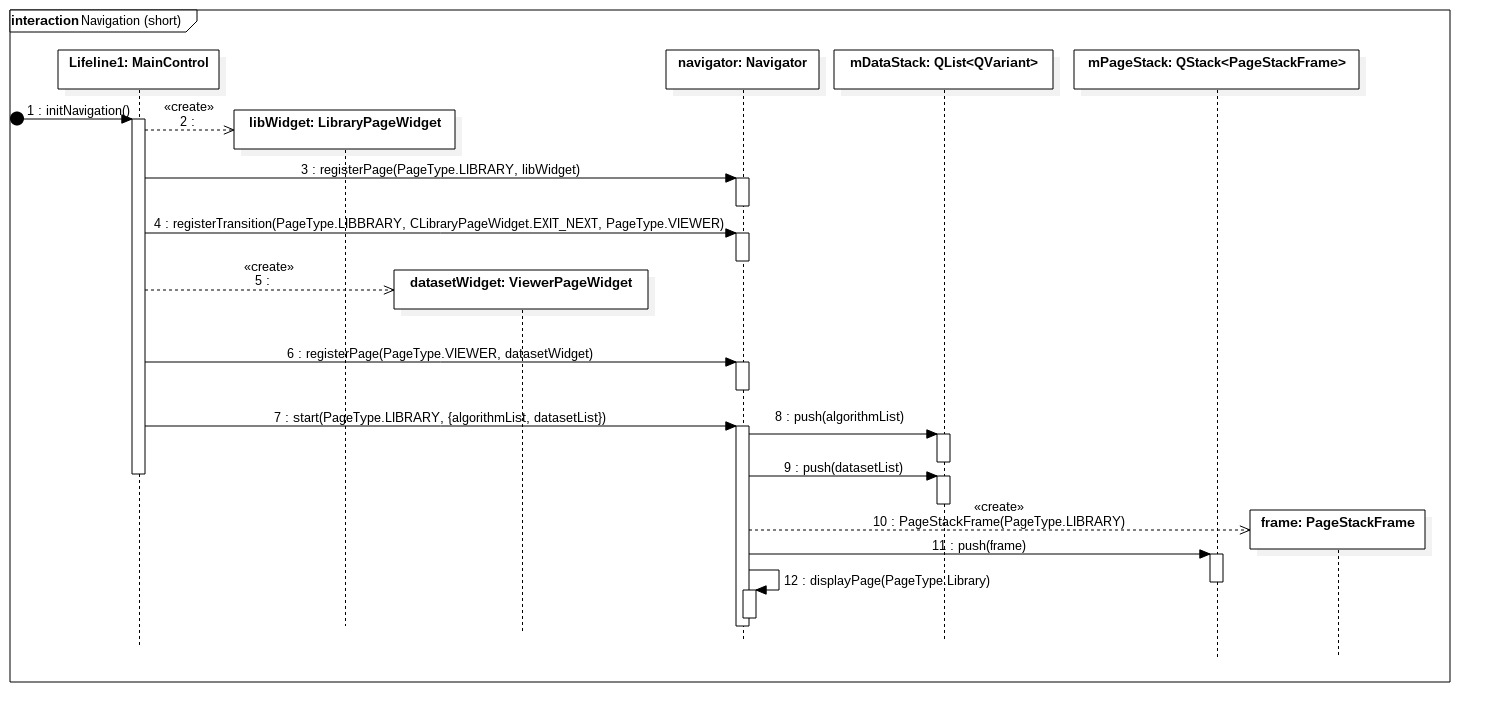
\includegraphics[width=\linewidth]{img/Sequenzdiagramme/Interaction}
\label{fig:Navigation init}
\end{figure}

Dieses Sequenzdiagramm beschreibt die Abläufe beim Programmstart, wenn MainControl die verschiedenen Komponenten initialisiert.

\begin{itemize}
	\item initNavigation() wird aufgerufen

	\item MainControl erstellt das LibraryPageWidget

	\item MainControl registriert das LibraryPageWidget und den Übergang zum ViewerPageWidget

	\item MainControl erstellt das ViewerPageWidget und registriert es beim Navigator

	\item Startet den Navigator mit LibraryView

	\item Fügt Suchdaten in den DataStack ein

	\item Erstellt ein PageStackFrame für die Library und fügt dieses zum PageStack hinzu

	\item Zeigt die Library an

\end{itemize}

\pagebreak

\subsection{Seitenwechsel}

\begin{figure}[H]
\centering
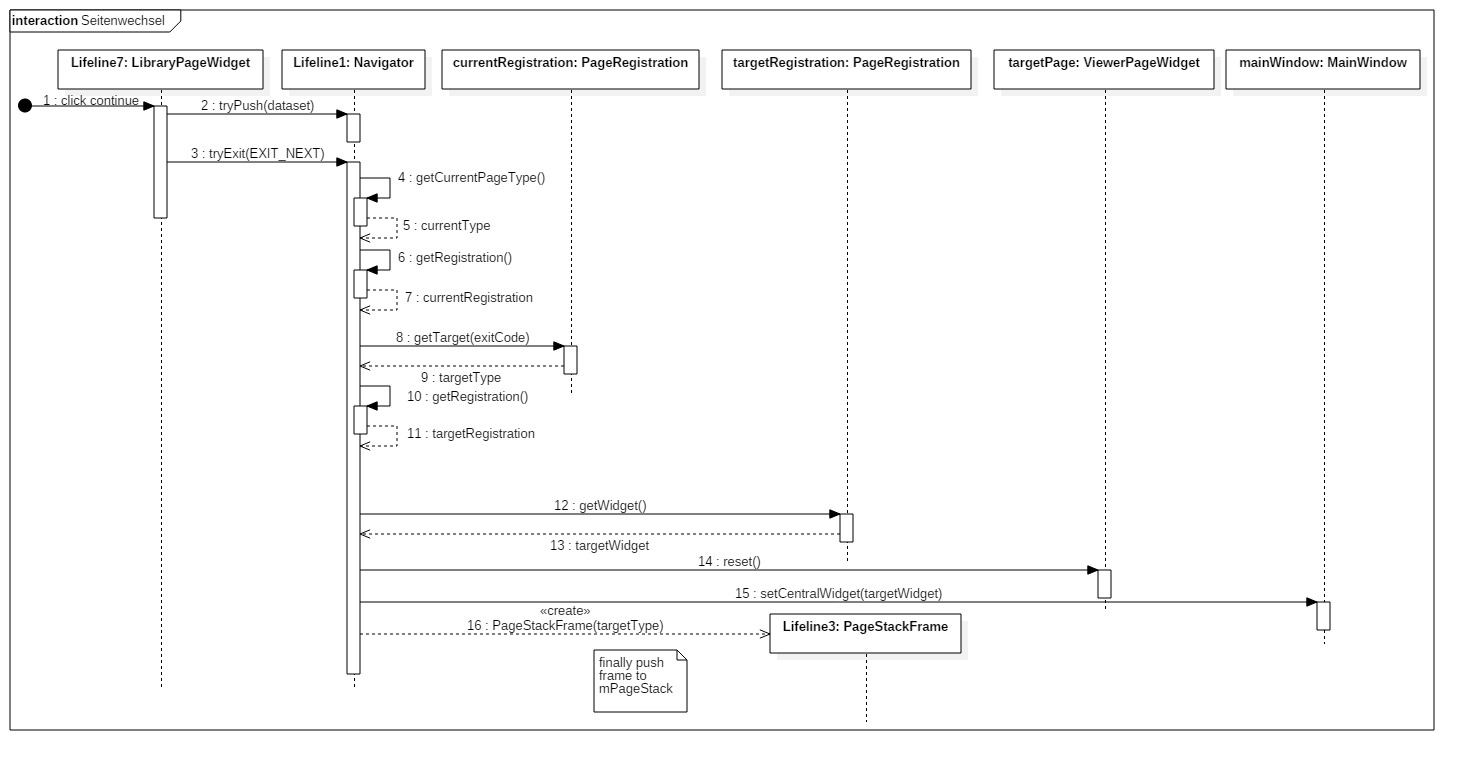
\includegraphics[width=\linewidth]{img/Sequenzdiagramme/Seitenwechsel}
\label{fig:seitenwechsel}
\end{figure}

Dieses Sequenzdiagramm beschreibt die Abläufe beim Seitenwechsel vom LibraryPageWidget zum ViewerPageWidget.

\begin{itemize}
	\item Benutzer klickt auf \enquote{weiter} (Library)

	\item Datensatz wird an Navigator gesendet

	\item LibraryPageWidget sendet Navigator einen Exit-Code, um die Seite zu wechseln

	\item Als PageType wird LIBRARY zurückgegeben. Die entsprechende PageRegistration wird ermittelt, aus der PageType die nächste Seite lesen lässt

	\item Aufruf der Funktion, ein PageWidget anhand von PageType anzuzeigen

	\item ViewerPageWidget wird wiederum aus PageRegistration abgelesen

	\item Der Navigator registriert das ViewerPageWidget als das PageWidget, das danach angezeigt werden soll. Das MainWindow erhält dieses.

\end{itemize}

\pagebreak

\subsection{Suche starten}

\begin{figure}[H]
\centering
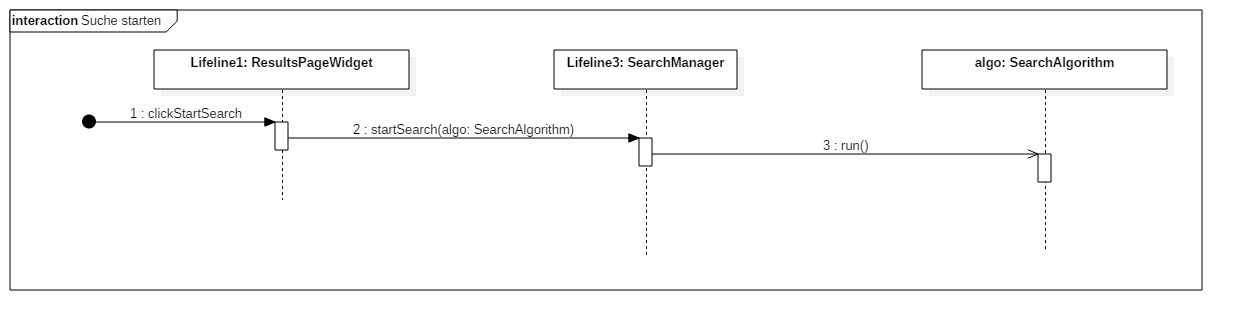
\includegraphics[width=\linewidth]{img/Sequenzdiagramme/SucheStarten}
\label{fig:sucheStarten}
\end{figure}
Nachdem der Benutzer den Button zum Start der Suche geklickt hat, übergibt das aktuelle PageWidget den Algorithmus an den SearchManager. Dieser startet die Suche.

\subsection{Suche terminieren}

\begin{figure}[H]
\centering
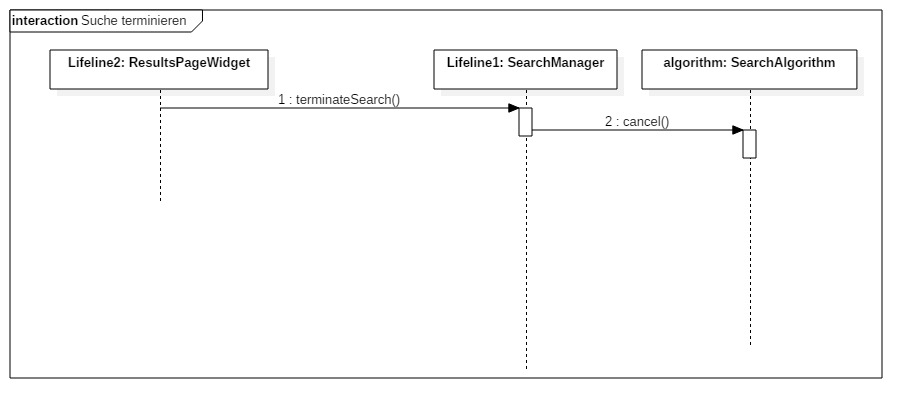
\includegraphics[width=\linewidth]{img/Sequenzdiagramme/SucheTerminieren}
\label{fig:sucheTerminieren}
\end{figure}
Das ResultsPageWidget veranlasst den SearchManager dazu, den Algorithmus zu beenden.

\subsection{Suchergebnis speichern}

\begin{figure}[H]
\centering
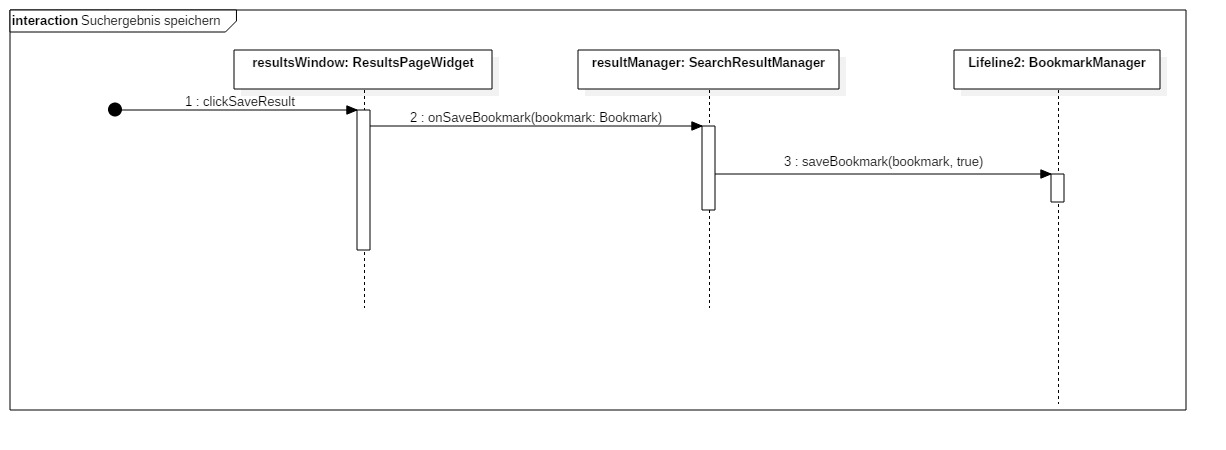
\includegraphics[width=\linewidth]{img/Sequenzdiagramme/SuchergebnisSpeichern}
\label{fig:suchergebnisSpeichern}
\end{figure}
Nachdem der Benutzer den Button zum Speichern des Suchergebnisses geklickt hat, übergibt das ResultsPageWidget dem SearchResultManager das Bookmark. Dieser ruft den BookmarkMangager zum Speichern auf.